% !TEX root = MAIN.tex


% !TEX root =  ../Main.tex

\subsection{Applicability of state-of-the-art solutions to space software}
\label{sec:background}

In this section, we discuss the applicability of state-of-the-art mutation testing optimizations in the context of space software. A detailed overview of mutation testing solutions and optimizations can be found in deliverable D1.

\subsubsection{Mutation adequacy and mutation score computation}

A mutant is said to be killed if at least one test case of the test suite fails when executed against the mutant.
Mutants that do not lead to the failure of any test case are said to be live.
Three conditions should hold for a test case to kill a mutant: reachability (i.e, the test case should execute the mutated statement), necessity (i.e., the test case should reach an incorrect intermediate state after executing the mutated statement), and sufficiency (i.e., the final state of the mutated program should differ from that of the original program)~\cite{offutt1997automatically}.

%The identification of killed and live mutants enables the definition of a mutation adequacy criterion as follow, a test suite is mutation-adequate if all mutants are killed by at least one test case of the test suite. Also, 
The mutation score, i.e., the percentage of killed mutants, measures the quality of a test suite quantitatively. Recent studies have shown that achieving a high mutation score improves significantly the fault detection capability of a test suite
~\cite{papadakis2018mutation}. 
%However, 
%to ensure better fault detection than a randomly selected subset of test cases, a test suite should achieve a very high mutation score~\cite{Chekam:17}.
%More precisely, they show that among randomly selected test suites, ranked based on mutation score and structural coverage, 
%only  the test suites in the top 5\% rank according to mutation score achieve a better fault detection rate than the ones ranked according to other criteria (e.g., branch coverage)~\cite{Chekam:17}. 
%The literature lacks studies on the identification of a mutation score threshold that guarantees achieving a fault detection rate higher than the one achieved by other adequacy criteria. 
However, a very high mutation score (i.e., above 0.75) is required to achieve a higher fault detection rate than the one obtained with other coverage criteria, such as statement and branch coverage~\cite{Chekam:17}.

The capability of a test case to kill a mutant also depends on the observability of the program state. To overcome the limitations due to observability, different strategies to identify killed mutants can be adopted; they are known as strong, weak, firm, and flexible mutation coverage~\cite{ammann2016introduction}. For space software, we suggest to rely on strong mutation because it is the only criterion that assesses the actual test suite's capability of detecting a fault; indeed, it relies on a mutation score that reflects the percentage of mutants identified by test failures. With the other mutation coverage criteria, a mutant is killed if the state of the mutant after the execution of the mutated statement differs from the one observed with the original code without any guarantee that either the erroneous values in state variables propagate or test oracles detect them. 




\subsubsection{Mutation Operators}
\label{sec:related:operators}

%% !TEX root =  ../Main.tex

\newcommand{\op}{\mathit{op}}
\newcommand{\ArithmeticSet}{ \texttt{+}, \texttt{-}, \texttt{*}, \texttt{/}, \texttt{\%} }
\newcommand{\LogicalSet}{ \texttt{&&}, \texttt{||} }
\newcommand{\RelationalSet}{ \texttt{>}, \texttt{>=}, \texttt{<}, \texttt{<=}, \texttt{==}, \texttt{!=} }
\newcommand{\BitWiseSet}{ \texttt{\&}, \texttt{|}, \land }
\newcommand{\ShiftSet}{ \texttt{>>}, \texttt{<<} }


\begin{table}[h]
\caption{Implemented set of mutation operators.}
\label{table:operators} 
\centering
\scriptsize
\begin{tabular}{|@{}p{4mm}@{}|@{}p{2cm}@{\hspace{1pt}}|@{}p{11.1cm}@{}|}
\hline
&\textbf{Operator} & \textbf{Description$^{*}$} \\
\hline
\multirow{7}{*}{\rotatebox{90}{\emph{Sufficient Set}}}&ABS               & $\{(v, -v)\}$	\\
\cline{2-3}
&AOR               & $\{(\op_1, op_2) \,|\, \op_1, \op_2 \in \{ \ArithmeticSet \} \land \op_1 \neq \op_2 \} $       \\
&    			  & $\{(\op_1, \op_2) \,|\, \op_1, \op_2 \in \{\texttt{+=}, \texttt{-=}, \texttt{*=}, \texttt{/=}, \texttt{\%} \texttt{=}\} \land \op_1 \neq \op_2 \} $       \\
\cline{2-3}
&ICR               & $\{i, x) \,|\, x \in \{1, -1, 0, i + 1, i - 1, -i\}\}$           \\
\cline{2-3}
&LCR               & $\{(\op_1, \op_2) \,|\, \op_1, \op_2 \in \{ \texttt{\&\&}, || \} \land \op_1 \neq \op_2 \}$            \\
&				  & $\{(\op_1, \op_2) \,|\, \op_1, \op_2 \in \{ \texttt{\&=}, \texttt{|=}, \texttt{\&=}\} \land \op_1 \neq \op_2 \}$            \\
&				  & $\{(\op_1, \op_2) \,|\, \op_1, \op_2 \in \{ \texttt{\&}, \texttt{|}, \texttt{\&\&}\} \land \op_1 \neq \op_2 \}$            \\
\cline{2-3}
&ROR               & $\{(\op_1, \op_2) \,|\, \op_1, \op_2 \in \{ \RelationalSet \}\}$            \\
&				  & $\{ (e, !(e)) \,|\, e \in \{\texttt{if(e)}, \texttt{while(e)}\} \}$ \\
\cline{2-3}
&SDL               & $\{(s, \texttt{remove}(s))\}$            \\
\cline{2-3}
&UOI               & $\{ (v, \texttt{--}v), (v, v\texttt{--}), (v, \texttt{++}v), (v, v\texttt{++}) \}$            \\   
\hline
\hline
\multirow{5}{*}{\rotatebox{90}{\emph{OODL}}}&AOD               & $\{((t_1\,op\,t_2), t_1), ((t_1\,op\,t_2), t_2) \,|\, op \in \{ \ArithmeticSet \} $       \\ 
\cline{2-3}
&LOD               & $\{((t_1\,op\,t_2), t_1), ((t_1\,op\,t_2), t_2) \,|\, op \in \{  \} \}$       \\ 
\cline{2-3}
&ROD               & $\{((t_1\,op\,t_2), t_1), ((t_1\,op\,t_2), t_2) \,|\, op \in \{ \RelationalSet \} \}$       \\ 
\cline{2-3}
&BOD               & $\{((t_1\,op\,t_2), t_1), ((t_1\,op\,t_2), t_2) \,|\, op \in \{ \BitWiseSet \} \}$       \\ 
\cline{2-3}
&SOD               & $\{((t_1\,op\,t_2), t_1), ((t_1\,op\,t_2), t_2) \,|\, op \in \{ \ShiftSet \} \}$       \\ 
%\hline
%COR               & $\{(\op_1, \op_2) \,|\, \op_1, \op_2 \in \{ \texttt{\&\&}, \texttt{||}, \land \} \land \op_1 \neq \op_2 \}$            \\
\hline
\hline
\multirow{3}{*}{\rotatebox{90}{\emph{Other}}}&LVR			& $\{(l_1, l_2) \,|\, (l_1, l_2) \in \{(0,-1), (l_1,-l_1), (l_1, 0), (\mathit{true}, \mathit{false}), (\mathit{false}, \mathit{true})\}\}$\\
&&\\
&&\\
\hline
\end{tabular}

$^{*}$Each pair in parenthesis shows how a program element is modified by the mutation operator. Th eleft element of the pair is replaced with the right element. We follow standard syntax~\cite{kintis2018effective}. Program elements are literals ($l$), integer literals ($i$), boolean expressions ($e$), operators ($\op$), statements ($s$), variables ($v$), and terms ( $t_i$, which might be either variables or literals).
\end{table}


Mutation testing introduces small syntactical changes into the code (source code or machine code) of a program through a set of mutation operators that simulate programming mistakes. 



The  \emph{sufficient set of operators} is widely used for conducting empirical evaluations ~\cite{offutt1996experimental,rothermel1996experimental,andrews2005mutation,kintis2017detecting}. 
%Initially defined by Offutt et al., the set has been extended to include newly defined operators.
The original sufficient set defined by Offutt et al. is composed of the following operators: absolute value insertion (ABS), arithmetic operator replacement (AOR), integer constraint replacement (ICR), logical connector replacement (LCR), relational operator replacement (ROR), and unary operator insertion (UOI)~\cite{offutt1996experimental}.
% operator and the \INDEX{statement deletion operator} (SDL).
Andrews et al.~\cite{andrews2005mutation} have included the 
\emph{statement deletion operator} (SSDL)~\cite{delamaro2014designing}, which ensures that every pointer-manipulation and field-assignment statement is properly tested. 
%Table~\ref{table:sufficient_operators} provides an overview of the operators belonging to the sufficient set.
%, thus targeting faults not simulated by the rest of the sufficient operators. In addition, recent research results show that the SDL operator is the most effective for fault detection~\cite{delamaro2014designing}. 
Deletion operators produce significantly less equivalent mutants~
\cite{delamaro2014designing,delamaro2014experimental}; also, 
test suites that kill mutants generated with OODL (deletion of arithmetic and relational operators) and SSDL (deletion of statements), kill a very high percentage of all mutants (e.g., 97\%)~\cite{delamaro2014experimental}. 
%However, since space software is different than other types of software systems (e.g., it includes functions to process signals, which are absent in Unix utilities), the pertinence of the mutation score generated with the SSDL operator should be evaluated.

%Operators used in other papers:
%
%Papadakis, M., Shin, D., Yoo, S., & Bae, D.-H. (2018). Are mutation scores correlated with real fault detection? a large scale empirical study on the relationship between mutants and real faults. 2018 IEEE/ACM 40th International Conference on Software Engineering (ICSE), 537?548.
%AOR (Arithmetic Operator Replacement), LOR (Logical Operator Replacement), COR (Conditional Operator Replacement), ROR (Relational Operator Replacement), ORU (Operator Replace- ment Unary), STD (STatement Deletion), and . Additional
%
%Chekam, T. T., Papadakis, M., Le Traon, Y., & Harman, M. (2017). An empirical study on mutation, statement and branch coverage fault revelation that avoids the unreliable clean program assumption. 2017 IEEE/ACM 39th International Conference on Software Engineering (ICSE), 597?608.
%The mutation tool includes the (large and varied) set of mutant operators used in previous research [4], [30], [49]. Specifically, we used mutants related to arithmetic, relational, conditional, logical, bitwise, shift, pointers and unary operators. We also used statement deletion, variable and constant replacement.



%(1) test suites that are mutation adequate (i.e., achieve 100\% mutation score) with respect to the sufficient set of operators also achieve a very high mutation score if we consider a larger set of mutation operators~\cite{offutt1996experimental}, 
The sufficient set of operators enables an accurate estimation of the mutation score of a test suite~\cite{siami2008sufficient}; furthermore, the mutation score computed with the sufficient set can estimate the fault detection rate (i.e., the portion of real faults discovered) of a test suite~\cite{andrews2005mutation}. 

Recent work has shown that, to maximize the detection of real faults, a set of operators to be used in addition to the sufficient set is the following: Conditional Operator Replacement (COR),
Literal Value Replacement (LVR), and Arithmetic Operator Deletion (AOD)~\cite{Kintis2018}. However, in C/C++ LVR is subsumed by 

An alternative to the sufficient set of operators is the generation of higher order mutants, which result from the application of multiple mutation operators for each mutation~\cite{jia2009higher,kintis2010evaluating,offutt1992investigations,papadakis2010empirical}. However, higher order mutants are of \emph{relatively lower strength than the first order ones}~\cite{papadakis2010mutation,papadakis2019mutation}, also there is \emph{lack of clear theory on which mutants are of some value}, and they may lead to redundant mutants~\cite{papadakis2019mutation}. For this reason, we focus our study on first order mutations.
% generated with the sufficient set.

%decreases consistently. 
%For instance, Papadakis and Malevris~\cite{papadakis2010empirical}, worked on a approach for higher order mutants for the C programming language that lead to a reduction of approximately 80-90\% of the generated equivalent mutants, with a fault detection ability loss only of 11-15\%. 
%
%
%that higher order mutants are of relatively lower strength than the first order ones
%
%Since modern space software is implemented in C and C++, thus sharing a degree of similarity with the case studies considered in the empirical evaluations for the sufficient set, we believe that the empirical findings concerning the sufficient set also hold for space software.

%rely on the sufficient set of operators.
%, to determine if results reported in the literature may generalize to the case of space software.
%For these reasons, we believe the sufficient set of operators to be necessary to be considered also for space software.

%% !TEX root =  ../Main.tex

\begin{table}
\scriptsize
\centering
\label{table:codeoperatorssummary}
\caption{Categories of mutation operators applicable to space software.}
\begin{tabular}{p{1.8cm}|p{5.4cm}}
\toprule
Operator Category & Description\\
\midrule
arithmetic & Includes operators that performs mutations on arithmetic expressions and assignments, usually these mutations replaces an element by an operator $op \in \{+, -, *, /, \%\}$. \\
bitwise & Includes operators that performs bitwise mutations on expressions and assignments, these mutations aims for replacing an element of an expression by an operator $op \in \{|, \&, \wedge, \sim\}$. \\
casts & Includes operators that work by mutating casting expressions.\\
constants & Includes operators that mutate constants in the code. \\
control-flow & Includes operators that modify and alter the execution flow of the running application.\\
coverage & Includes operators that mutate the code in such a way that the static structure of the code (e.g., branches) is likely covered during execution.\\
deletion & Includes operators that mutate the code by deleting statements, operators, constants and variables.  \\
floating points & Includes operators working on floating point comparison (FPC).\\
function calls & Includes operators that mutate function calls and their components (e.g., signature and parameters).\\
logical & Includes operators that performs logical mutations on expressions and assignments; these mutations replace an element of an expression by an operator $op \in \{\&\&, \|, !\}$.\\
variable references & Includes operators mutating different types of variable references in the code (e.g., scalars, arrays and pointers).\\
shift & Includes operators that performs shift mutations on expressions and assignments; usually, these mutations replace an element by an operator $op \in \{<<, <<<, >>, >>>\}$.\\
SQL & Includes operators that modify SQL clauses, SQL \texttt{NULL} operators, and SQL \texttt{WHERE} operators.\\
statements & Includes operators performing syntactical changes at a statement-level granularity.\\
strings & Includes operators that performs mutations on variables of string type.\\
structures & Includes operators that mutate C/C++ structures.\\
higher-order & Includes operators for generating second- and higher-order mutants. These strategies combine first order mutants to simulate more complex faults, motivated by a desire to capture subtle faults~\cite{jia2009higher}. Usually, each operator of this category introduce a strategy on how to combine first order operators to form a higher-order one. For example, the \emph{RMix} operator combines any two randomly selected first order operator to generate a higher-order mutant. \\
system-configuration & Includes operators that perform mutations at a system-configuration level; usually, these mutation operators aim to cause faults concerning the configuration of the system itself.\\
system-level & Includes operators that performs mutations at a system-level; usually, these mutation operators aim to cause faults concerning the integration of system components. \\
ADA expressions & Includes operators that work by modifying expressions in the ADA programming language. \\
ADA operands & Includes operators that perform mutations by replacing operands in ADA expressions (e.g., variables, constants, records, arrays, pointers).\\
ADA tasks & Includes operators that mutate ADA code at the granularity of tasks and aim to trigger problems related to concurrency in the program.\\
\bottomrule
\end{tabular}
\end{table}
%
%In addition to the sufficient set of operators, we can group the mutation operators targeting space software (i.e., software implemented in C/C++) into XX categories. Table~\ref{} provides an overview of these additional categories of operators along with references and a discussion of the reasons why they should be selected or avoided when applying mutation testing to space software.

%% !TEX root =  ../Main.tex

\newcommand{\op}{\mathit{op}}
\newcommand{\ArithmeticSet}{ \texttt{+}, \texttt{-}, \texttt{*}, \texttt{/}, \texttt{\%} }
\newcommand{\LogicalSet}{ \texttt{&&}, \texttt{||} }
\newcommand{\RelationalSet}{ \texttt{>}, \texttt{>=}, \texttt{<}, \texttt{<=}, \texttt{==}, \texttt{!=} }
\newcommand{\BitWiseSet}{ \texttt{\&}, \texttt{|}, \land }
\newcommand{\ShiftSet}{ \texttt{>>}, \texttt{<<} }


\begin{table}[h]
\caption{Implemented set of mutation operators.}
\label{table:operators} 
\centering
\scriptsize
\begin{tabular}{|@{}p{4mm}@{}|@{}p{2cm}@{\hspace{1pt}}|@{}p{11.1cm}@{}|}
\hline
&\textbf{Operator} & \textbf{Description$^{*}$} \\
\hline
\multirow{7}{*}{\rotatebox{90}{\emph{Sufficient Set}}}&ABS               & $\{(v, -v)\}$	\\
\cline{2-3}
&AOR               & $\{(\op_1, op_2) \,|\, \op_1, \op_2 \in \{ \ArithmeticSet \} \land \op_1 \neq \op_2 \} $       \\
&    			  & $\{(\op_1, \op_2) \,|\, \op_1, \op_2 \in \{\texttt{+=}, \texttt{-=}, \texttt{*=}, \texttt{/=}, \texttt{\%} \texttt{=}\} \land \op_1 \neq \op_2 \} $       \\
\cline{2-3}
&ICR               & $\{i, x) \,|\, x \in \{1, -1, 0, i + 1, i - 1, -i\}\}$           \\
\cline{2-3}
&LCR               & $\{(\op_1, \op_2) \,|\, \op_1, \op_2 \in \{ \texttt{\&\&}, || \} \land \op_1 \neq \op_2 \}$            \\
&				  & $\{(\op_1, \op_2) \,|\, \op_1, \op_2 \in \{ \texttt{\&=}, \texttt{|=}, \texttt{\&=}\} \land \op_1 \neq \op_2 \}$            \\
&				  & $\{(\op_1, \op_2) \,|\, \op_1, \op_2 \in \{ \texttt{\&}, \texttt{|}, \texttt{\&\&}\} \land \op_1 \neq \op_2 \}$            \\
\cline{2-3}
&ROR               & $\{(\op_1, \op_2) \,|\, \op_1, \op_2 \in \{ \RelationalSet \}\}$            \\
&				  & $\{ (e, !(e)) \,|\, e \in \{\texttt{if(e)}, \texttt{while(e)}\} \}$ \\
\cline{2-3}
&SDL               & $\{(s, \texttt{remove}(s))\}$            \\
\cline{2-3}
&UOI               & $\{ (v, \texttt{--}v), (v, v\texttt{--}), (v, \texttt{++}v), (v, v\texttt{++}) \}$            \\   
\hline
\hline
\multirow{5}{*}{\rotatebox{90}{\emph{OODL}}}&AOD               & $\{((t_1\,op\,t_2), t_1), ((t_1\,op\,t_2), t_2) \,|\, op \in \{ \ArithmeticSet \} $       \\ 
\cline{2-3}
&LOD               & $\{((t_1\,op\,t_2), t_1), ((t_1\,op\,t_2), t_2) \,|\, op \in \{  \} \}$       \\ 
\cline{2-3}
&ROD               & $\{((t_1\,op\,t_2), t_1), ((t_1\,op\,t_2), t_2) \,|\, op \in \{ \RelationalSet \} \}$       \\ 
\cline{2-3}
&BOD               & $\{((t_1\,op\,t_2), t_1), ((t_1\,op\,t_2), t_2) \,|\, op \in \{ \BitWiseSet \} \}$       \\ 
\cline{2-3}
&SOD               & $\{((t_1\,op\,t_2), t_1), ((t_1\,op\,t_2), t_2) \,|\, op \in \{ \ShiftSet \} \}$       \\ 
%\hline
%COR               & $\{(\op_1, \op_2) \,|\, \op_1, \op_2 \in \{ \texttt{\&\&}, \texttt{||}, \land \} \land \op_1 \neq \op_2 \}$            \\
\hline
\hline
\multirow{3}{*}{\rotatebox{90}{\emph{Other}}}&LVR			& $\{(l_1, l_2) \,|\, (l_1, l_2) \in \{(0,-1), (l_1,-l_1), (l_1, 0), (\mathit{true}, \mathit{false}), (\mathit{false}, \mathit{true})\}\}$\\
&&\\
&&\\
\hline
\end{tabular}

$^{*}$Each pair in parenthesis shows how a program element is modified by the mutation operator. Th eleft element of the pair is replaced with the right element. We follow standard syntax~\cite{kintis2018effective}. Program elements are literals ($l$), integer literals ($i$), boolean expressions ($e$), operators ($\op$), statements ($s$), variables ($v$), and terms ( $t_i$, which might be either variables or literals).
\end{table}

\subsubsection{Compile-time Scalability}
\label{sec:compile:time}

%The time spend in compiling mutants depend on the number of mutants to be compiled. 
%The time spent in compiling mutants depends on the number of invocations of the compiler.
%For this reason, \emph{mutant schemata} include all the mutations into a single executable~\cite{untch1993mutation} thus needing only a single  compiler pass. 

To reduce the number of invocations of the compiler to one, \emph{mutant schemata} include all the mutations into a single executable~\cite{untch1993mutation}. 
With mutant schemata, the mutations to be tested are selected at run-time through configuration parameters. They may lead to a compilation speed-up of 300\% \cite{papadakis2010automatic}. 


Another solution to address compile-time scalability issues consists of mutating machine code  (e.g., binary code~\cite{becker2012xemu}, assembly language~\cite{crouzet2006sesame},
Java~\cite{ma2006mujava}, 
 and
.NET~\cite{derezinska2011object} bytecode) thus avoiding the execution of the compilation process after creating a mutant. 
%Empirical results show that the generation of mutants for compiled code requires only 50\% of the time required by a traditional mutation testing process applied to source code~\cite{derezinska2011object,becker2012xemu}.
A common solution consists of mutating the
 LLVM Intermediate Representation (IR) \cite{hariri2016evaluating}, 
which enables the development of mutants that work with multiple programming languages~\cite{hariri2019comparing} and facilitates the integration of optimizations based on dynamic program analysis~\cite{denisov2018mull}.


Unfortunately, the mutation of machine code 
may lead to mutants that are not representative of real faults because impossible to generate with the source code~\cite{schuler2009efficient}.
In the case of IR mutation, a part of these mutants can be automatically identified~\cite{denisov2018mull}; however,
the number of generated mutants tend to be higher at the IR level than at the source code level, which may reduce scalability~\cite{hariri2019comparing}.
 In addition, we have encountered three problems that prevented the application of 
 mutation testing tools based on  LLVM IR to our case study systems.
First, space software relies on compiler pipelines (e.g., RTEMS~\cite{RTEMS}) that include architecture-specific optimizations not supported by LLVM. 
Second, there is no guarantee that the executables generated by LLVM are equivalent to those produced by other compilers.
%, which may 
%undermine the validity of mutation testing assessment 
% (e.g., mutants may fail because of errors introduced by the compiler). 
 Third, efficient toolsets based on LLVM often  perform mutations dynamically~\cite{denisov2018mull}, which is infeasible when the software under test needs to be executed within a dedicated simulator (this is the case of the ESAIL case study system).




\subsubsection{Runtime Scalability}
\label{sec:scalability}

A straightforward mutation testing process consists of executing the full test suite against every mutant, which may lead to scalability problems in the case of a large SUT.
Simple optimizations that can be applied to space software consist of (S1) stopping the execution of the test suite when the mutant has been killed, (S2) executing only those test cases that cover the mutated statements~\cite{delamaro1996proteum}, and (S3) rely on time thresholds to automatically detect infinite loops introduced by mutation~\cite{papadakis2019mutation}. 

\emph{Split-stream} execution consists of generating a modified version of the SUT that creates multiple processes (one for each mutant) only when the mutated code is reached \cite{king1991fortran,tokumoto2016muvm}, thus saving time and resources. Unfortunately, it cannot be applied in the case of space software that needs to be run on simulators because, in general, the hosting simulator cannot be forked by the hosted SUT.

A practical solution consists of  randomly selecting only a portion of the generated mutants~\cite{zhang2010operator,gopinath2015hard,zhang2013operator}. 
%
%Zhang et al. \cite{zhang2010operator} demonstrated that a test suite that is capable of killing 50\% of the mutants results in killing more than 99\% of all mutants.
%
%Gopinath et al \cite{gopinath2015hard} show that the mutation score obtained for a subset of the mutants is representative of the mutation score obtained by considering all the mutants. Best results were obtained by considering 1 000 mutants. The number of mutants to consider is independent of the total number of available mutants. With 1 000 mutants, the error in the prediction of the mutation score was 7\% with a probability of 95\%.
% 
Zhang et al. \cite{zhang2013operator} empirically demonstrated that a random selection of 5\% of the mutants is sufficient for 
%correctly predicting the mutation score. 
estimating, with high confidence, the mutation score obtained with the complete mutants set.
Also,
they show that sampling mutants uniformly across different program elements (e.g., functions) %i.e., to have a same percentage of mutants selected for every function/methods) 
leads to a more accurate mutation score prediction than sampling mutants globally in a random fashion. It also fares better than uniformly distributing the sampled mutants across different mutation operators. In the presence of large software systems that lead to hundred thousand mutants, random mutation testing is the only viable solution. However, for large systems, a percentage of mutants below 5\% might need to be selected.

Other solutions aim to sort test cases to augment the likelihood of executing first the ones that kill the mutants thus preventing the execution of most of the test suite and save time.
Solutions that simply prioritize faster test cases~\cite{just2012using}
 may not be useful with system-level test suites whose test cases have homogeneous execution time.
Approaches that rely on data-flow analysis to identify and prioritize the test cases that likely satisfy the killing conditions~\cite{papadakis2011automatically} may not scale with large space systems.
Solutions that combine multiple coverage measures need to be adapted in order 
to be feasible in the space context~\cite{zhang2013faster}.
Current work~\cite{zhang2013faster} combines three criteria: (1) the number of times the mutated statement is exercised by the test case (multiple iterations over a same statement are likely performed with a diverse set of variable values and thus have higher probability to kill the mutant), (2) the proximity of the mutated statement to the end of the test case (closer ones have higher chances of satisfying the sufficiency condition), and (3) the percentage of mutants belonging to the same class file of the mutated statement that were already killed by the test case (test cases that kill multiple mutants likely exercise the SUT with a diverse set of inputs). 
Criterion (3) is also used to reduce the test suite size (i.e., to select only the test cases above a given threshold). 
Unfortunately, only criterion (1) might be applicable for space software; indeed, criterion (2) might be ineffective with system test cases whose results are checked after long executions, while criterion (3) might be inefficient when only a random selection of mutants is executed. 






%For \INDEX{test case reduction}, the idea is to remove those test cases that are somehow redundant (e.g., test cases that when removed from the test suites do not change the mutation score).
%Usaola et al. \cite{usaola2012reduction} proposed a greedy algorithm that iteratively selects  the test cases that kill most of the mutants that were not killed by the previously selected test cases. 
%%\DONE{No change to do here. However please keep them in mind for the current work.}
%Shi et al. \cite{shi2014balancing} assessed the effects of reducing the size of test suites with an experiment on 18 projects with a total of 261\,235 test cases. Their results show that \emph{it is possible to maintain constant the mutation score and reduce test suite size without loss in the \emph{fault detection rate}}. 
%On the same line, Zhang et al. \cite{zhang2013faster} suggest to define a subset of tests of the original test suite and to run the mutants against the subset, their assumption is that if the mutants cannot be killed by the subset also the original test suite will not be able to kill the mutants.
%
%
%




\subsubsection{Detection of Equivalent Mutants}

Despite identifying equivalent mutants is an undecidable problem~\cite{madeyski2013overcoming,Bugg:Correctness:82}, several heuristics to partially address the problem had been developed. 

The simplest solution consists of relying on \emph{trivial compiler optimisations}~\cite{papadakis2015trivial, kintis2017detecting,papadakis2019mutation}, i.e., compile both the mutants and the original program with compiler optimisations enabled and determine that the mutant is equivalent when their executable code match. In the case of programs written in C, compiler optimisations can reduce the total number of mutants by 28\%~\cite{kintis2017detecting}.


Solutions that identify equivalent mutants based on symbolic execution~\cite{holling2016nequivack}, bounded model checking~\cite{riener2011test}, and program slicing ~\cite{harman2001relationship} are unlikely to scale with large systems because of the limitations of static analysis. Also, their implementation often relies on LLVM, which may prevent their applicability to space software (see Section~\ref{sec:compile:time}).

Alternative solutions rely on comparing the data collected at runtime when testing the original software and the mutants~\cite{grun2009impact,schuler2010covering,schuler2013covering}.
%A large number of program classes presenting different statement coverage in test suites executions with the original and the mutated code is an indicator for  mutants to be non-equivalent~\cite{grun2009impact}.
The most extensive empirical study on the topic shows that non-equivalent mutants can be detected by counting the number of methods (mutated method excluded) that, for at least one test case, either (1) have statements that are executed at a different frequency with the mutant, (2) generate at least one different return value, or (3) are invoked at a different frequency~\cite{schuler2013covering}. To determine if a mutant is non-equivalent, it is possible to define a threshold indicating the smallest number of methods with such characteristics. A threshold of one identifies non-equivalent mutants with an average precision above 70\% and an average recall above 60\%. It outperforms more sophisticated methods relying on dynamic invariants~\cite{schuler2009efficient}.
Values above one slightly improve precision but make recall drop (e.g., recall is below 50\% for a threshold of five); also, the proper threshold value may depend on the size of the test suite. 

Concerning the applicability of coverage-based methods to space software, it is worth noting that, because of real-time constraint, it might be feasible to collect only coverage frequency data, which, however, lead to results close to the ones achieved by including all the three criteria~\cite{schuler2013covering}.
Unfortunately, the  results reported in the literature concern a small number of mutants (i.e., 140) for Java software; further empirical evaluations might be needed to determine if these findings hold for C/C++ space software. 
In particular, the identification of coverage differences across the whole software might be ineffective when the SUT is exercised with system test cases that may lead to non-deterministic internal software behaviours (e.g., because of interrupt handlers). Finally, we notice that although coverage-based approaches might be an effective solutions to detect mutants that are not-equivalent (i.e., two executions showing different coverage are likely semantically different) they might be inappropriate to identify equivalent mutants. Indeed, not-equivalent mutants that are not exercised with an appropriate set of inputs may lead to the same coverage. For example, the condition $(x >= 0)$ leads to the same coverage of $(x > 0)$ if not tested with $(x=0)$. For this reason, a mutation score computed by including only such non-equivalent mutants might be higher than the real mutation score, which might be dangerous if mutation testing is used to assess the quality of test suites for safety critical software.

\subsubsection{Detection of Redundant Mutants}

Redundant mutants are either \emph{duplicate}, i.e., mutants that are equivalent with each other but not equivalent to the original program, or \emph{subsumed}, i.e., mutants that are not equivalent with each other but are killed by the same test cases. 

We observe that duplicate mutants can be detected by relying on the same approaches adopted for equivalent mutants. 

To identify subsumed mutants, Shin et al. suggest augmenting the test suite with additional test cases so that each mutant can trigger a test failure that cannot be observed with other mutants~\cite{Shin:TSE:DCriterion:2018}. 
The augmented test suites have a higher
 fault detection rate than test suites that simply satisfy mutation coverage; however, with large software systems the approach might be infeasible because of the lack of scalable test inputs generation approaches.


\subsubsection{Summary}

We aim to rely on the sufficient set of operators because it has been successfully used to generate a mutation score that accurately estimate the fault detection rate for software written in C and C++, typical languages of space software systems.
Based on recent results, we should extend the sufficient set with COR, and AOD.

To speed up mutation testing by reducing the number of mutants, the SSDL operator alone might be considered. However, the confidence of the results generated with the SSDL operator should be evaluated.

Among compile time optimizations, only mutant schemata appear to be feasible.
Simple runtime scalability optimizations (i.e., S1, S2, and S3 in Section~\ref{sec:scalability}) are feasible in the case of space software. Other feasible solutions are the ones relying on mutant sampling and coverage metrics. However, the confidence of the results generated for mutant sampling rates below 5\% should be evaluated. Furthermore, code coverage metrics that are feasible for space software need to be defined.

Equivalent mutants can be identified through trivial compiler optimizations and the analysis of coverage differences; however, coverage metrics that are robust with respect to non-deterministic internal software behaviours should be developed.





% !TEX root =  ../Main.tex
\subsection{Space Software Mutation Testing Process}
\label{sec:approach}

\begin{figure}[h!]
\begin{center}
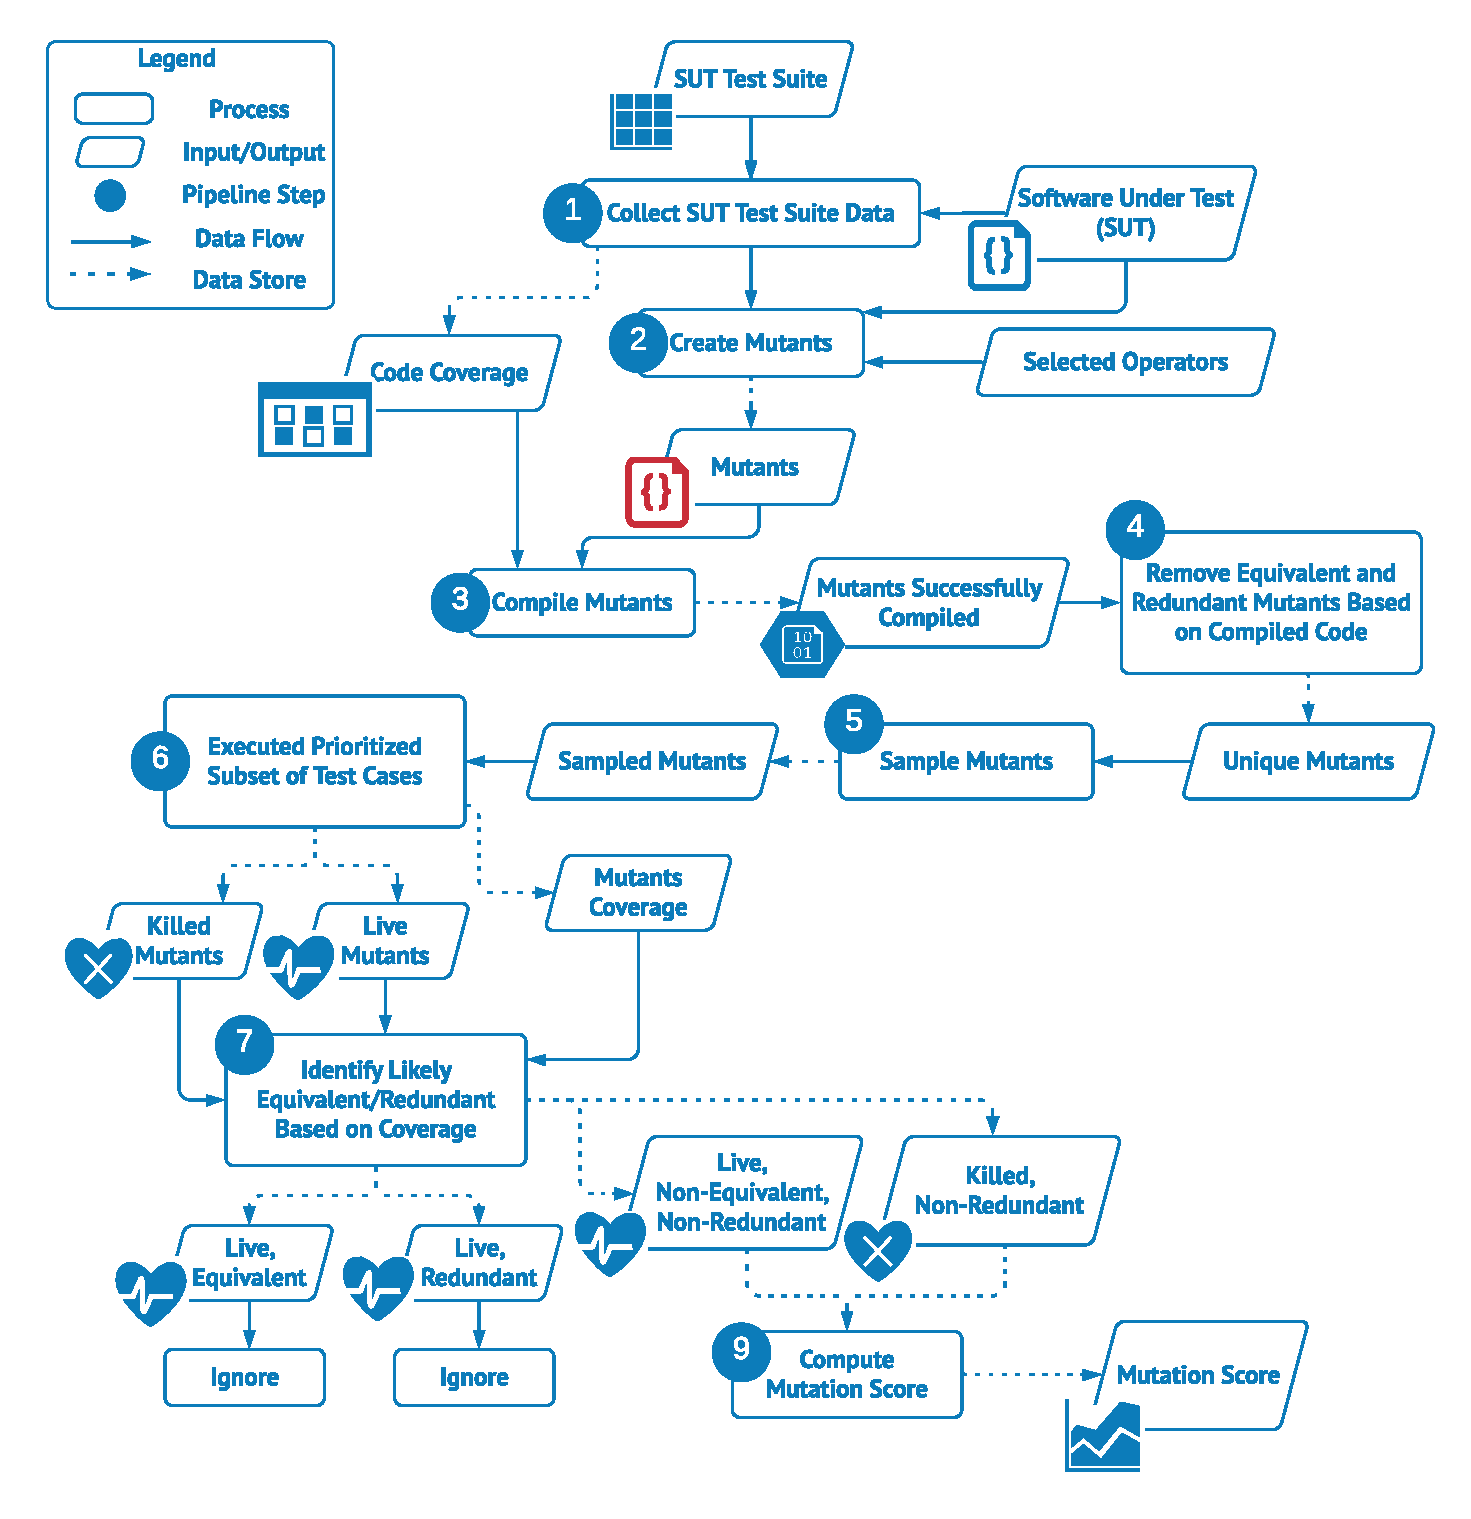
\includegraphics[width=\textwidth]{images/MT}
\caption{Overview of the proposed Mutation Testing Pipeline}
\label{fig:approach}
\end{center}
\end{figure}

Figure~\ref{fig:approach} provides an overview of the mutation testing process that we propose, namely Scalable Mutation Testing for Space Software  (\APPR). We describe each step in the following paragraphs. 

\subsubsection{Step 1}

In Step 1, the test suite is executed against the software under test (SUT) and code coverage information is collected. 
More precisely, we rely state-of-the art code coverage tools such as gcov~\cite{GCOV} and Vector CAST~\cite{VectorCAST} 
to record the number of times each line of code of the SUT has been exercised by a test case.

\subsubsection{Step 2}

In Step 2, we automatically generate mutants for the SUT by relying on a set of selected mutation operators.
In \APPR, based on the considerations provided in Section~\ref{sec:related:operators}, we rely on an extended sufficient set of mutation operators, which are listed in Table~\ref{table:sufficient_operators}.
In addition, in our experiments, we evaluate the feasibility of relying only on the SDL operators instead of the whole sufficient set of operators.

% !TEX root =  ../Main.tex

\newcommand{\op}{\mathit{op}}
\newcommand{\ArithmeticSet}{ \texttt{+}, \texttt{-}, \texttt{*}, \texttt{/}, \texttt{\%} }
\newcommand{\LogicalSet}{ \texttt{&&}, \texttt{||} }
\newcommand{\RelationalSet}{ \texttt{>}, \texttt{>=}, \texttt{<}, \texttt{<=}, \texttt{==}, \texttt{!=} }
\newcommand{\BitWiseSet}{ \texttt{\&}, \texttt{|}, \land }
\newcommand{\ShiftSet}{ \texttt{>>}, \texttt{<<} }


\begin{table}[h]
\caption{Implemented set of mutation operators.}
\label{table:operators} 
\centering
\scriptsize
\begin{tabular}{|@{}p{4mm}@{}|@{}p{2cm}@{\hspace{1pt}}|@{}p{11.1cm}@{}|}
\hline
&\textbf{Operator} & \textbf{Description$^{*}$} \\
\hline
\multirow{7}{*}{\rotatebox{90}{\emph{Sufficient Set}}}&ABS               & $\{(v, -v)\}$	\\
\cline{2-3}
&AOR               & $\{(\op_1, op_2) \,|\, \op_1, \op_2 \in \{ \ArithmeticSet \} \land \op_1 \neq \op_2 \} $       \\
&    			  & $\{(\op_1, \op_2) \,|\, \op_1, \op_2 \in \{\texttt{+=}, \texttt{-=}, \texttt{*=}, \texttt{/=}, \texttt{\%} \texttt{=}\} \land \op_1 \neq \op_2 \} $       \\
\cline{2-3}
&ICR               & $\{i, x) \,|\, x \in \{1, -1, 0, i + 1, i - 1, -i\}\}$           \\
\cline{2-3}
&LCR               & $\{(\op_1, \op_2) \,|\, \op_1, \op_2 \in \{ \texttt{\&\&}, || \} \land \op_1 \neq \op_2 \}$            \\
&				  & $\{(\op_1, \op_2) \,|\, \op_1, \op_2 \in \{ \texttt{\&=}, \texttt{|=}, \texttt{\&=}\} \land \op_1 \neq \op_2 \}$            \\
&				  & $\{(\op_1, \op_2) \,|\, \op_1, \op_2 \in \{ \texttt{\&}, \texttt{|}, \texttt{\&\&}\} \land \op_1 \neq \op_2 \}$            \\
\cline{2-3}
&ROR               & $\{(\op_1, \op_2) \,|\, \op_1, \op_2 \in \{ \RelationalSet \}\}$            \\
&				  & $\{ (e, !(e)) \,|\, e \in \{\texttt{if(e)}, \texttt{while(e)}\} \}$ \\
\cline{2-3}
&SDL               & $\{(s, \texttt{remove}(s))\}$            \\
\cline{2-3}
&UOI               & $\{ (v, \texttt{--}v), (v, v\texttt{--}), (v, \texttt{++}v), (v, v\texttt{++}) \}$            \\   
\hline
\hline
\multirow{5}{*}{\rotatebox{90}{\emph{OODL}}}&AOD               & $\{((t_1\,op\,t_2), t_1), ((t_1\,op\,t_2), t_2) \,|\, op \in \{ \ArithmeticSet \} $       \\ 
\cline{2-3}
&LOD               & $\{((t_1\,op\,t_2), t_1), ((t_1\,op\,t_2), t_2) \,|\, op \in \{  \} \}$       \\ 
\cline{2-3}
&ROD               & $\{((t_1\,op\,t_2), t_1), ((t_1\,op\,t_2), t_2) \,|\, op \in \{ \RelationalSet \} \}$       \\ 
\cline{2-3}
&BOD               & $\{((t_1\,op\,t_2), t_1), ((t_1\,op\,t_2), t_2) \,|\, op \in \{ \BitWiseSet \} \}$       \\ 
\cline{2-3}
&SOD               & $\{((t_1\,op\,t_2), t_1), ((t_1\,op\,t_2), t_2) \,|\, op \in \{ \ShiftSet \} \}$       \\ 
%\hline
%COR               & $\{(\op_1, \op_2) \,|\, \op_1, \op_2 \in \{ \texttt{\&\&}, \texttt{||}, \land \} \land \op_1 \neq \op_2 \}$            \\
\hline
\hline
\multirow{3}{*}{\rotatebox{90}{\emph{Other}}}&LVR			& $\{(l_1, l_2) \,|\, (l_1, l_2) \in \{(0,-1), (l_1,-l_1), (l_1, 0), (\mathit{true}, \mathit{false}), (\mathit{false}, \mathit{true})\}\}$\\
&&\\
&&\\
\hline
\end{tabular}

$^{*}$Each pair in parenthesis shows how a program element is modified by the mutation operator. Th eleft element of the pair is replaced with the right element. We follow standard syntax~\cite{kintis2018effective}. Program elements are literals ($l$), integer literals ($i$), boolean expressions ($e$), operators ($\op$), statements ($s$), variables ($v$), and terms ( $t_i$, which might be either variables or literals).
\end{table}

To automatically generate mutants, we have extended SRCIRor~\cite{hariri2018srciror} to include all the mutation operators of the sufficient set. After mutating the original source file, our extension saves the mutated source file and keeps track of the mutation applied. 

\subsubsection{Step 3}
\label{codeDriven:stepThree}

In Step 3, we compile mutants by relying on the build system of the SUT. To this end, we have developed a toolset that, for each mutated source file: (1) backs-up the original source file, (2) renames the mutated source file as the original source file, (3) runs the build system (e.g., executes the command \texttt{make}), (4) copies the generated executable mutant in a dedicated folder, (5) restores the original source file. 

Build systems create one object file for each source file to be compiled and then link these object files together into the final executable. For this reason, since we modify at most two source files for each mutant (i.e., the mutated file and the file restored from previous mutation), we can reuse almost all the compiled object files in subsequent compilation runs, thus speeding up the compilation of multiple mutants. Some preliminary experiments conducted with our case study systems have shown that additional compile-time optimizations (e.g., mutant schemata) are not necessary to make the compilation of mutants feasible.

\MREVISION{C-P-24}{Mutants that lead to compilation errors are discarded. Concerning compilation warnings, we assume the build system of the SUT has been properly configured; more precisely, if the system should compile without warnings, the compiler is expected to be configured to treat warnings as errors otherwise mutants that lead to warning are retained.}

\subsubsection{Step 4}

In Step 4, we rely on trivial compiler optimizations to identify and remove equivalent and redundant mutants. 
\MREVISION{C-P-15}{We aim to enable all the available optimizations (e.g., \texttt{-O3} or \texttt{-Ofast} in GCC).}
If the SUT is already configured to be compiled with optimizations enabled, Step 4 consists of first computing the SHA-512 hash summary of all the mutant and original executables and then compare all the generated hash summaries. Hash comparison enables us to (1) determine the presence of equivalent mutants (i.e., mutants having the same hash of the original executable), and (2) identify duplicate mutants (i.e., mutants with the same hash). %Mutants that are identified as being either equivalent and redundant mutants are ignored in the following steps of \APPR. 
Equivalent and redundant mutants are discarded.
The outcome of Step 4 is a set of \emph{unique mutants}, i.e., mutants with compiled code that differs from the original software and any other mutant.

If the SUT should not be compiled with compiler optimizations enabled, we identify equivalent and redundant mutants by re-executing Step 3 with compiler optimizations enabled and then apply Step 4.
%The executables generated by this additional run of Step 3 are used only to identify equivalent mutants, not to evaluate the SUT test suite, which is based on executables compiled without optimizations (otherwise test cases may fail).

\subsubsection{Step 5}

In Step 5, we sample the mutants to be executed to compute the mutation score. This optimization is based on the results of Zhang et al.~\cite{zhang2013operator}, who compare eight strategies for sampling mutants. In our work, we consider two strategies. The first is the \emph{baseline sampling} strategy, which consists of randomly selecting $r\%$ mutants from the complete mutants set. The second is the \emph{method-based sampling} strategy, which is the best performing strategy in \cite{zhang2013operator} and consists of sampling mutants evenly across all functions of the SUT, i.e., sampling $r\%$ mutants from each set of mutants generated inside a same function.

%In Section~\ref{}, we evaluate which of these sampling strategies lead to mutation score


\subsubsection{Step 6}

In Step 6, we execute a prioritized subset of test cases. 
We execute test cases in sequence, and we select only the ones that satisfy 
the reachability condition (i.e., cover the mutated statement).
Similarly to the approach of Zhang et al. \cite{zhang2013faster}, we define the order of execution of test cases based on their likelihood of killing a mutant. However, we redefined the criteria for the selection of test cases because of the inapplicability of the ones proposed by Zhang et al. (see Section~\ref{sec:scalability}).


\MREVISION{C-P-46}{We execute only covered statements assuming that the test suite is optimal with respect to code coverage. More precisely, we addume that if a statement is not covered there is a good reason for it (e.g., it depends on hardware). 
If a statement is not covered by the test suite, there is no chance that a mutant generated in the non-covered statement can be possibly detected by any test case. 
If the test suite does not reach the required coverage there is no reason to perform mutation testing, because is already known that the test suite is not good.}
%\EMPH{When computing the mutation score, is it fare to not count those not-covered lines?}
%Yes, is it fare because mutation testing assess the quality of existing test suites, and considering non-covered statements would be out of the scope of the technique. Also, including non-covered statements into the mutation score, would not let us to assess correctly the quality of the existing test suite.
%\EMPH{Maybe the approach would be to run the test augmentation process to provide test cases for the missing statements?}
%Yes, the same tools used for test augmentation can be used. We can run them. The main difference is that oracles  for the generated test cases should be manually specified (in the case of test augmentation we may derive the oracle based on the values generated by KLEE/CBMC). However, the evaluation of these generated test suites through mutation testing address a different research question than the one of the project; i.e., we would evaluate test automation tools instead of manual test suites.




%However, we notice that such optimization may not be sufficient when test suites are particularly large; indeed, prioritizing test cases may not be sufficient to reduce execution time. For example, live mutants may lead to the execution of a large number of test cases when almost all the test cases of the test suite exercise the mutated statement. 


To reduce the number of test cases to be executed with a mutant, 
we should first execute the ones that more likely satisfy the necessity condition. 
More precisely, the next test case to be executed in a sequence should be the one that exercises the mutated statement with variable values not observed before. 
Unfortunately, in our context, the size of the SUT and its real-time constraints prevent us from recording all the variable values processed during testing. 

To determine if two test case executions exercise the mutated statement with diverse variable values, we rely on code coverage.
% as a surrogate indicator of  variable values diversity.
%diversity in values assigned to the variables used in a statement. 
Indeed, a difference in the set of instructions being covered by two test cases that exercise the mutated statement may depend on the values used in the mutated statement. 
However, since the behaviour of the whole software depends on all the executed software instructions, we reduce the scope of our code coverage analysis 
%to the file containing the source code of the mutated function. 
to the mutated function, its callers, and its callees.
%to maximize the chances that a change in the behaviour of the software depends on the values used in a mutated statement, we determine that two executions likely exercise a mutated statement with diverse values by focussing on the coverage of 
%the mutated function, its callers, and its callees.
A reduced scope is effective in determining behavioural differences based on the analysis of variable valuations~\cite{Pastore:VART:2014}.

%Since related work focuses on either statement coverage or the frequency of execution of a statement, 
Following related work, we have identified two possible criteria to characterize test case executions based on code coverage:
\begin{itemize}
\item[C1] Identify the set $C_t$ of source code statements being covered by the test case.
%\item[C2] Identify the set of unique pairs $\langle\mathit{statement},\mathit{arity}\rangle$, where $\mathit{statement}$ is a unique identifier for the source code statement, and $\mathit{arity}$ is a symbol (i.e., $1$ or $*$) indicating if the statement has been covered one or more times.
\item[C2] Derive a vector whose values capture the number of times each monitored statement had been covered.
\end{itemize}

We have identified distance metrics that determine how dissimilar two test cases are, and, consequently how likely they exercise the mutated statement with different values. In the case of C1 we rely on the Jaccard and Ochiai index, which are two similarity indexes for binary data successfully used to compare program executions based on code coverage~\cite{Zou:Ochiai:2019,Keller:Jaccard:2017,Briand:2019}. Given two test cases $T_A$ and $T_B$, the Jaccard  ($D_J$) and the Ochiai ($D_O$) distance are computed as follows:

$D_J(T_a,T_b)=\frac{|C_a \cap C_b|}{|C_a \cup C_b|}$ \hspace{5mm} $D_O(T_a,T_b)=1-\frac{|C_a \cap C_b|}{\sqrt{|C_a| * |C_b|}}$, 
$C_a$ and $C_b$ are the set of coverage items exercised by the test cases $T_a$ and $T_b$, respectively.

In the case of C2, we compute the distance between two test cases by relying on the euclidean distance ($D_E$) and the cosine similarity distance ($D_C$), two popular distance metrics used in machine learning. Given two vectors $V_A$ and $V_B$ that capture the number of times each statement has been covered by test cases $T_A$ and $T_B$, the distances $D_E$ and $D_C$ can be computed as follows:

$D_E=\sqrt{\sum_{i=1}^{n}(A_i-B_i)^2}$ 
$D_C= \frac{\sum_{i=1}^{n}A_i*B_i}{\sqrt{\sum_{i=1}^{n}{A_i}^2}*\sqrt{\sum_{i=1}^{n}{B_i}^2}}$,
%Their main difference is that cosine similarity is used when the magnitude of the vectors should not matter.
$A_i$ and $B_i$ refer to the number of times the i-th statement had been covered by test cases $T_A$ and $T_B$, respectively.

Figure~\ref{alg:prioritize} shows the pseudocode of our algorithm for selecting and prioritizing test cases. It generates as output
a prioritized test suite (i.e., \emph{PTS}) that consists of a subset of the test cases that exercise the mutated statement (Line~\ref{alg:prioritize:select}).
Based on the findings of Zhang et al. \cite{zhang2013faster}, we first select the test case that exercises the mutated statement more times (Line~\ref{alg:prioritize:first}) \MREVISION{C-P-17}{ and add it to the prioritized test suite (Line~\ref{alg:prioritize:add}).}
Then, the next selected test case is the one with the largest distance from the closest test case belonging to the set of test cases already selected (Lines~\ref{alg:prioritize:selectStart} to~\ref{alg:prioritize:selectEnd}). 
%is most different than any other test case already included in the prioritized test suite.

%Then, since we aim to maximize test cases diversity, the next selected test case should be the one that is most different than any other test case already included in the prioritized test suite.
%For this reason, for each test case $n$ not selected yet (Line~\ref{alg:prioritize:notSel}), we identify the test case $t$ showing the most similar coverage (i.e., the one with the minimal distance $d$, Line~\ref{alg:prioritize:minD}). We then select the test case $n$ with the highest distance from its closest test case (Lines~\ref{alg:prioritize:selectStart} to~\ref{alg:prioritize:selectEnd}). 

The algorithm iterates as long as it identifies a test case that exercises 
the program instructions differently than the test cases already selected (Line~\ref{alg:prioritize:until}).

Test cases are then executed in the selected order. During the execution we collect code coverage information and identify killed and live mutants.

% !TEX root =  ../Main.tex

\newcommand{\INDA}{10}
\newcommand{\INDB}{15}
\newcommand{\INDC}{5}

%\vspace{-3mm}
\begin{figure}[tb]

\begin{algorithmic}[1]

%\footnotesize
\scriptsize
\Require \emph{TS}, the test suite of the software under test
\Require \emph{Cov}, coverage information, for each test case
\Require \emph{ms}, the mutated statement
\Ensure \emph{PTS}, a list of test cases to be executed, sorted by priority
% (source inputs, follow-up inputs, output data).

\State $\mathit{TS}_m \gets$ subset of $\mathit{TS}$ that cover the mutated statement $\mathit{ms}$, based on \emph{Cov} \label{alg:prioritize:select}
\State $\mathit{PTS} \gets \mathit{new} \mathit{list}$ \textcolor{darkgray}{//this list is initially empty}
\State $\mathit{PTS} \gets$ based on \emph{Cov} select from $\mathit{TS_m}$ the test case $t$ that exercises $\mathit{ms}$ more times \label{alg:prioritize:first}
\State $\mathit{PTS} \gets \mathit{PTS} \cup t$ \textcolor{darkgray}{//include first the test case selected above}  \label{alg:prioritize:add}

\State \textbf{repeat} \label{alg:prioritize:repeat}
\State \hspace{\INDC mm} \textbf{for each} $n$ in the set ($\mathit{TS}_m$ - $\mathit{PTS}$) \textcolor{darkgray}{, which is the set of test cases not already added to $\mathit{PTS}$} \label{alg:prioritize:notSel}
\State \hspace{\INDA mm} \textbf{for each} $t$ in $\mathit{PTS}$
\State \hspace{\INDB mm} compute the distance between $t$ and $n$
\State \hspace{\INDA mm} identify $t_n$ i.e., the test case $t$ with the minimal $d$ \label{alg:prioritize:minD}
\State \hspace{\INDC mm} among all the $t_n$ identified, select the one with the highest distance $d$ \label{alg:prioritize:selectStart}
\State \hspace{\INDC mm} \textbf{if} $d > 0$ \textcolor{darkgray}{//there is at least a test case with a different coverage}
\State \hspace{\INDA mm} \textcolor{darkgray}{//note: $n$ is the test case in the set ($\mathit{TS}_m$ - $\mathit{PTS}$) closer to $t_n$}
\State \hspace{\INDA mm} $\mathit{PTS} \gets \mathit{PTS} \cup n$ \label{alg:prioritize:selectEnd}
\State \textbf{until} $d > 0$ \label{alg:prioritize:until}


\end{algorithmic}
\vspace{-3mm}
\caption{Algorithm for prioritizing test cases}
%\vspace{-0.2cm}
\label{alg:prioritize}
\end{figure}




\subsubsection{Step 7}


In Step 7, we identify likely equivalent and likely redundant mutants by relying on code coverage information.

Differently from related work~\cite{schuler2013covering}, since the size of a program may impact on the number of statement that present coverage differences because of non-determinism, 
to identify equivalent and redundant mutants through a threshold, instead of relying on the absolute number of methods/statements presenting differences in code coverage, we compute normalized distances based on the distance metrics $D_J$, $D_O$, $D_E$, and $D_C$. 

%To identify equivalent mutants, we select the
A mutant is considered non-equivalent when the distance from the original program is above the threshold $T_E$, for at least one test case.
Similarly, a mutant is considered non-redundant when the distance from every other mutants is above the threshold $T_R$, for at least one test case.

\MREVISION{C-P-19}{Figure~\ref{alg:nonEquivalent:nonRedeundat} shows the algorithm for detecting non-equivalent and non-redundant mutants.
It first identify among the list of killed mutants all the non-redundant ones (Line~\ref{alg:equivalent:KNR}).
Then it identifies the non-equivalent mutants among the list of live mutants (Line~\ref{alg:equivalent:LNE}).
Finally, it further filters the list of non-equivalent mutants to keep only the ones that appear to be non-redundant (Line~\ref{alg:equivalent:LNENR}).}

% !TEX root =  ../Main.tex

\renewcommand{\INDA}{5}
\renewcommand{\INDB}{10}
\renewcommand{\INDC}{15}
\newcommand{\INDD}{20}
\newcommand{\INDE}{25}

\renewcommand{\Comment}[1]{\textcolor{darkgray}{\textit{//#1}}}

%\vspace{-3mm}
\begin{figure}[tb]

\begin{algorithmic}[1]

%\footnotesize
\scriptsize
\Require \emph{D}, the distance function to use to identify equivalent/duplicate mutants
\Require \emph{KM}, list of killed mutants
\Require \emph{LM}, list of live mutants
\Require $\mathit{Cov}_O$, coverage information for all the test cases, for the original program
\Require $\mathit{Cov}_M$, coverage information for all the executed test cases, for every mutant
\Require \emph{TS}, list of test cases
\Require \emph{TR}, test results, for all the executions
\Ensure \emph{KNR}, a list of killed, non-duplicate  mutants
\Ensure \emph{LNENR}, a list of live, non-equivalent, non-duplicate mutants
% (source inputs, follow-up inputs, output data).

%\State $\mathit{TS}_m \gets$ subset of $\mathit{TS}$ that cover the mutated statement $\mathit{ms}$, based on \emph{Cov} \label{alg:equivalent:select}
%\State $\mathit{PTS} \gets \mathit{new} \mathit{list}$ \textcolor{darkgray}{//this list is initially empty}
%\State $\mathit{PTS} \gets$ based on \emph{Cov} select from $\mathit{TS_m}$ the test case $t$ that exercises $\mathit{ms}$ more times \label{alg:equivalent:first}
\State $\mathit{KNR} \gets \mathit{identifyNonDuplicateMutants(} \mathit{KM}, \mathit{TS}, \mathit{TR}, \mathit{Cov}_M)$ \label{alg:equivalent:KNR}
\State $\mathit{LNE} \gets \mathit{identifyNonEquivalentMutants(} \mathit{LNR}, \mathit{TS}, \mathit{Cov}_M, \mathit{Cov}_O)$ \label{alg:equivalent:LNE}
\State $\mathit{LNENR} \gets \mathit{identifyDuplicateMutants(} \mathit{LNE}, \mathit{TS}, \mathit{Cov}_M)$ \label{alg:equivalent:LNENR}


\Procedure{identifyNonDuplicateMutants}{$\mathit{M},\mathit{TS},\mathit{TR},\mathit{Cov}_M$}\Comment{$M$ is a  list of mutants, $\mathit{TS}$, $\mathit{TR}$, and $\mathit{Cov}_M$ are defined above}
\State $\mathit{NR} \gets \mathit{empty} \mathit{set}$
\State $\mathit{k1} \gets $ extract and remove first element of M
\State $\mathit{NR} \gets \mathit{NR} \cup \mathit{k1}$
\While {$\mathit{M}$ not empty}
\State $\mathit{k2} \gets $ extract and remove first element of M
\For {mutant $k1$ in $\mathit{NR}$}
\State $\mathit{duplicate}=\mathit{TRUE}$
\For {test case $t$ in $\mathit{TS}$}
\If {$t$ has different result in $k1$ and $k2$ }
\State $\mathit{duplicate}=\mathit{FALSE}$
\State \textbf{break}
\Else
\State $\mathit{cov}_{k1t} \gets $ extract coverage information for test case $t$ executed with mutant $k1$
\State $\mathit{cov}_{\mathit{k2}t} \gets $ extract coverage information for test case $t$ executed with mutant $k2$
\If {$D(\mathit{cov}_{k1t},\mathit{cov}_{\mathit{k2}t}) > T_R$ }
\State $\mathit{duplicate}=\mathit{FALSE}$
\State \textbf{break}
\EndIf
\EndIf
\EndFor
\If {$\mathit{duplicate}==\mathit{FALSE}$}
\State \textbf{break} \Comment{No need to compare with all the mutants if we know that it is not duplicate}
\EndIf
\EndFor
\If {$\mathit{duplicate}==\mathit{FALSE}$}
\State $\mathit{NR} \gets \mathit{NR} \cup \mathit{k2}$
\EndIf
\EndWhile
\State \textbf{return} $\mathit{NR}$
\EndProcedure


\Procedure{identifyNonEquivalentMutants}{$\mathit{M},\mathit{TS},\mathit{Cov}_M,\mathit{Cov}_O$}\Comment{$M$ is a  list of mutants, $\mathit{TS}$, and $\mathit{Cov}_M$, and $\mathit{Cov}_O$ are defined above}
\State $\mathit{NE} \gets \mathit{empty} \mathit{set}$
\While {$\mathit{M}$ not empty}
\State $\mathit{m} \gets $ extract and remove first element of M

\For {test case $t$ in $\mathit{TS}$}
\State $\mathit{cov}_{m} \gets $ extract coverage information for test case $t$ executed with mutant $m$
\State $\mathit{cov}_{o} \gets $ extract coverage information for test case $t$ executed with original program

\If {$D(\mathit{cov}_{m},\mathit{cov}_{o}) > T_E$ }
\State $\mathit{equivalent}=\mathit{FALSE}$
\State \textbf{break}
\EndIf

\EndFor

\If {$\mathit{equivalent}==\mathit{FALSE}$}
\State $\mathit{NE} \gets \mathit{NE} \cup \mathit{m}$
\EndIf

\EndWhile

\State \textbf{return} $\mathit{NE}$
\EndProcedure



%
%
%\State \hspace{\INDA mm} \textbf{if} $\mathit{KM}$ not empty
%\State \hspace{\INDB mm} compute the distance between $t$ and $n$
%\State \hspace{\INDA mm} identify $t_n$ i.e., the test case $t$ with the minimal $d$ \label{alg:equivalent:minD}
%\State \hspace{\INDC mm} among all the $t_n$ identified, select the one with the highest distance $d$ \label{alg:equivalent:selectStart}
%\State \hspace{\INDC mm} \textbf{if} $d > 0$ \textcolor{darkgray}{//there is at least a test case with a different coverage}
%\State \hspace{\INDA mm} \textcolor{darkgray}{//note: $n$ is the test case in the set ($\mathit{TS}_m$ - $\mathit{PTS}$) closer to $t_n$}
%\State \hspace{\INDA mm} $\mathit{PTS} \gets \mathit{PTS} \cup n$ \label{alg:equivalent:selectEnd}
%\State \textbf{until} $d > 0$ \label{alg:equivalent:until}


\end{algorithmic}
\vspace{-3mm}
\caption{Algorithm for identifying non-equivalent and non-duplicate mutants}
%\vspace{-0.2cm}
\label{alg:nonEquivalent:nonRedeundat}
\end{figure}



\subsubsection{Step 8}

The mutation score is computed as the ratio between the number of live, non-equivalent and non-redundant mutants  and the overall number of non-equivalent, non-redundant mutants identified in Step 7:

$\mathit{mutation}\ \mathit{score} = \frac{|\mathit{LNENR}|}{|\mathit{LNENR}|+|\mathit{KNR}|}$,
$\mathit{LNE}$ is the number of live, non-equivalent, non-redundant mutants,
$\mathit{KNR}$ is the number of killed non-redundant mutants.

%Similarly,
%
%obof at lest one test case with respect
%
%
%The code coverage difference between the mutant and the original program is represented by a \textit{threshold T\%}, a difference of code coverage over a certain T\% indicates that both versions are not equivalent.





%\subsection{Mutation Operators}
%\label{sec:operators}
%
%Mutation testing introduces small syntactical changes into the code of a program 
%%\MREVISION{C8}{(source code, intermediate representation, or executable code)} 
%through a set of mutation operators.
%The goal of the mutation operators is to simulate artificial faults by systematically introducing  simple syntax changes \MREVISION{C9}{based on errors that programmers typically make. 
%Each of these operators model a specific type of fault. For example, the use of a wrong variable is a fault; the \emph{variable references} category of operators, introduced later in this section, model this type of fault.}
%
%
%\TODO{verify which set we are considering}
%
%Table~\ref{table:codeoperatorssummary} provides the  category of the mutation operators that will be implemented in FAQAS along with their relevance. All the relevant operators will be implemented in the FAQAS toolset. The others might be implemented if empirical evaluation, code inspection, and discussion with engineers show that might be necessary.
%
%The relevant set coincides with the \INDEX{sufficient set of operators}~\cite{rothermel1996experimental,andrews2005mutation}.
%This set is composed of the following operators: absolute value insertion (ABS), arithmetic operator replacement (AOR), logical connector replacement (LCR), relational operator replacement (ROR) the unary operator insertion (UOI) operator and the \INDEX{statement deletion operator} (SDL).
%We refer to the sufficient set of operators identified by Andrews et al.~\cite{andrews2005mutation}. With respect to previous work, this set includes also the the \INDEX{statement deletion operator} (SDL). The SDL operator has been included because it ensures that every pointer-manipulation and field-assignment statement is properly tested, thus targeting faults not simulated by the rest of the sufficient operators. In addition, recent research results show that the SDL operator is the most effective for fault detection~\cite{delamaro2014designing}. 
%
%
%We selected the \INDEX{sufficient set of operators}, because
%there is empirical evidence that \emph{(1) test suites that are \INDEX{mutation adequate} (i.e., achieve 100\% mutation score) with respect to the sufficient set of operators also achieve a very high mutation score if we consider a larger set of mutation operators}~\cite{offutt1996experimental}, \emph{(2) the sufficient set of operators enables an \EMPH{accurate estimation of the mutation score} of a test suite}~\cite{siami2008sufficient}, and (3) the mutation score can estimate the \INDEX{fault detection rate} (i.e., the number of real faults discovered) of a test suite~\cite{andrews2005mutation}.
%
%
%\TODO{Unclear what is the column number of operators}
%
%% !TEX root =  ../MutationTestingSurvey.tex



\setlength\LTleft{0pt}
\setlength\LTright{0pt}
\small 
\begin{longtable}{@{\extracolsep{\fill}}|l|l|l|l|@{}}
\caption{\normalsize Summary of the code-driven mutation operators applicable to space-context software. On the last column \emph{Relevance for FAQAS} the symbols mean: ** \textit{relevant}, * \textit{potentially relevant}, * \textit{NA} Not Applicable to FAQAS case studies.}
\label{table:codeoperatorssummary} \\
\hline

	\textbf{\begin{tabular}[c]{@{}l@{}}Operator\\Category\end{tabular}}	&	\textbf{\begin{tabular}[c]{@{}l@{}}Number of\\Operators\end{tabular}}	&	\textbf{Context}	&	\textbf{Relevance for FAQAS}\\

\hline
	Arithmetic			&	14	&	C/C++; LLVM-IR; OO; SQL; Simulink	& **\\
	Bitwise				&	15	&	C/C++; LLVM-IR; OO; SQL 			& **\\
	Casts				&	1	&	C/C++ 								& *\\
	Constants			&	8	&	C/C++; LLVM-IR; OO; Simulink 		& **\\
	Control-flow		&	11	&	C/C++ & *\\
	Coverage			&	6	&	C/C++; ADA & *\\
	Deletion			&	5	&	C/C++; LLVM-IR; OO & **\\
	Logical				&	10	&	C/C++; LLVM-IR; OO; Simulink & **\\
	Relational			&	5	&	C/C++; LLVM-IR; OO; SQL; Simulink & **\\
	Variable References	&	12	&	C/C++; LLVM-IR; OO; SQL; Simulink & **\\
	Shift				&	10	&	C/C++; OO & *\\
	Statements			&	21	&	C/C++; ADA; Simulink & *\\
	Structures			&	3	&	C/C++ & *\\
	Strings				&	7	&	C/C++ & *\\
	Function Calls		&	38	&	C/C++; LLVM-IR; SQL & *\\
	Floating Points		&	6	&	C/C++ & *\\
	Memory Operations	&	9	&	C/C++ & *\\
	System-level		&	14	&	OO & *\\
	Object-Oriented		&	36	&	C/C++; OO & *\\
	SQL					&	27	&	SQL & NA\\
	ADA					&	47	&	ADA & NA\\
\bottomrule                                                             
\end{longtable}
\normalsize

